\documentclass[12pt, a4paper]{article}
\usepackage{graphicx} % Required for inserting images
\usepackage[paper=a4paper,top=1in,bottom=1in,right=1in,left=1in]{geometry}% http://ctan.org/pkg/geometry
\usepackage{amsmath, xparse}
\setcounter{MaxMatrixCols}{20}
\usepackage{caption}
\usepackage[framed, numbered]{matlab-prettifier}
\usepackage{longtable}
\usepackage{float}
\usepackage{amsmath}
\usepackage{tikz}
\usepackage{pgfplots}
\usepackage{comment}

\setlength\parindent{0pt}
\numberwithin{equation}{section}



\begin{document}

\begin{titlepage}
   \begin{center}
       
\includegraphics[width=0.25\textwidth]{img/metu.png}\\
       \vspace*{1cm}
       \Large
       \textbf{MIDDLE EAST TECHNICAL UNIVERSITY}\\
       \vspace{0.05cm}
       \textbf{DEPARTMENT OF MECHANICAL ENGINEERING}\\
       \vspace{1.2cm}
       \textbf{ME 310 – NUMERICAL METHODS}\\
       \textbf{SPRING 2022}\\
       \vspace{3cm}
       \text{HOMEWORK 2}\\
       \vspace{2cm}
       \text{Muhammed Rüstem ŞEVİK - 2446888}

       \vfill
       
       \small
       I understand that this is an individual assignment. I affirm that I have not given or received
any unauthorized help on this assignment, and that this work is my own.
            
       \vspace{0cm}

            
   \end{center}
\end{titlepage}

\newpage
    \renewcommand{\contentsname}{Table of Contents}
    \tableofcontents
    \listoffigures
\newpage

\section{Introduction}

In this assignment, students are given a range of tasks that involve different types of regression and interpolation. The second question focuses on regression, requiring students to analyze linear and non-linear regression. Similarly, the sixth question requires them to explore generalized regression. Moving on to the eighth question, students are expected to employ Newton and Lagrange methods to fit a polynomial. Additionally, they are asked to perform natural cubic spline interpolation within the same question. Lastly, the thirteenth question involves bi-quadratic interpolation. These exercises offer students an opportunity to enhance their understanding of regression and interpolation techniques. By completing these tasks, students will gain valuable practical knowledge in these mathematical concepts.

\section{Body}
\subsection{Question 2}


\subsubsection{Part A}
To fit the model $y = Ate^{Bt}$ to the data, we can take the natural logarithm of both sides:
\begin{equation}
    \ln(y) = \ln(Ate^{Bt}) = \ln(A) + \ln(t) + Bt
\end{equation}

Let $Y = \ln(y) - ln(t)$, $X = t$. We have a linear equation of the form:

\begin{equation}
    Y = \ln(A) + BX
\end{equation}

We can apply linear regression to find the values of $\ln(A)$ and $B$.

Using the given data points:

\begin{table}[!ht]
    \centering
    \begin{tabular}{ccccc}
    \hline
        $t$ & $X$ & $\ln(t)$ & $\ln(y)$ & $Y$ \\ \hline
        1 & 1 & 0 & 2.079 & 2.079 \\ 
        2 & 2 & 0.693 & 2.509 & 1.8165 \\ 
        3 & 3 & 1.099 & 2.740 & 1.6422 \\
        4 & 4 & 1.386 & 2.821 & 1.4351 \\ 
        5 & 5 & 1.609 & 2.839 & 1.2296 \\ 
        6 & 6 & 1.792 & 2.760 & 0.9683 \\ 
        7 & 7 & 1.946 & 2.721 & 0.7754 \\ 
        8 & 8 & 2.079 & 2.639 & 0.5596 \\ \hline
    \end{tabular}
\end{table}

Let's calculate the necessary sums:
\begin{equation}
\begin{aligned}
n &= 8 \\
\sum X &= 1 + 2 + 3 + 4 + 5 + 6 + 7 + 8 = 36 \\
\sum Y &= 2.0794 + 1.8165 + 1.6422 + 1.4351 + 1.2296 \\
&\quad + 0.9683 + 0.7754 + 0.5596
 = 10.5061 \\
\sum X^2 &= 1^2 + 2^2 + 3^2 + 4^2 + 5^2 + 6^2 + 7^2 + 8^2 = 204 \\
\sum XY &= (1 \cdot 2.079) + (2 \cdot 1.8165) + (3 \cdot 1.6422) + (4 \cdot 1.4351) \\
&\quad + (5 \cdot 1.2296) + (6 \cdot 0.9683) + (7 \cdot 0.7754) + (8 \cdot 0.5596) = 38.2418 \\
\end{aligned}
\end{equation}

Now, let's find the values of $\ln(A)$ and $B$ using the formulas:
\begin{equation}
\begin{aligned}
B &= \frac{n\sum XY - \sum X \sum Y}{n\sum (X)^2 - (\sum X)^2} \\
\ln(A) &= \frac{\sum Y - B\sum (X)}{n}
\end{aligned}
\end{equation}


Substituting the values, we find:
\begin{equation}
\begin{aligned}
B &= - 0.215 \\
\ln(A) &= 2.28
\end{aligned}
\end{equation}


Thus, the linearized model is:
\begin{equation}
    \ln(y) = 2.28 + \ln(t) - 0.215t
\end{equation}
Taking the exponential of both sides:
\begin{equation}
    y = 9.77te^{-0.215t}
\end{equation}
To estimate the concentration at $t = 16$ hours, we substitute $t = 16$ into the model:

\begin{equation}
    y(16) = 5.0124
\end{equation}
The $r^2$ value:

Calculate the total sum of squares (SST):
\begin{equation}
\text{SST} = \sum (y_i - \bar{y})^2
\end{equation}
where $y_i$ is the observed concentration, and $\bar{y}$ is the mean concentration.

Calculate the sum of squares of residuals (SSR):
\begin{equation}
\text{SSR} = \sum (y_i - f(t_i))^2
\end{equation}
where $f(t_i)$ is the predicted concentration obtained from the regression equation $y = 9.77te^{-0.215t}$.
Calculate the coefficient of determination $r^2$:
\begin{equation}
r^2 = 1 - \frac{\text{SSR}}{\text{SST}}
\end{equation}

In this formulation, we can substitute the appropriate values and perform the calculations using the derived coefficient values from the least-squares fit to obtain the $r^2$ value.
$$ r^2 = 0.99096$$
\begin{figure}[H]
  \centering
  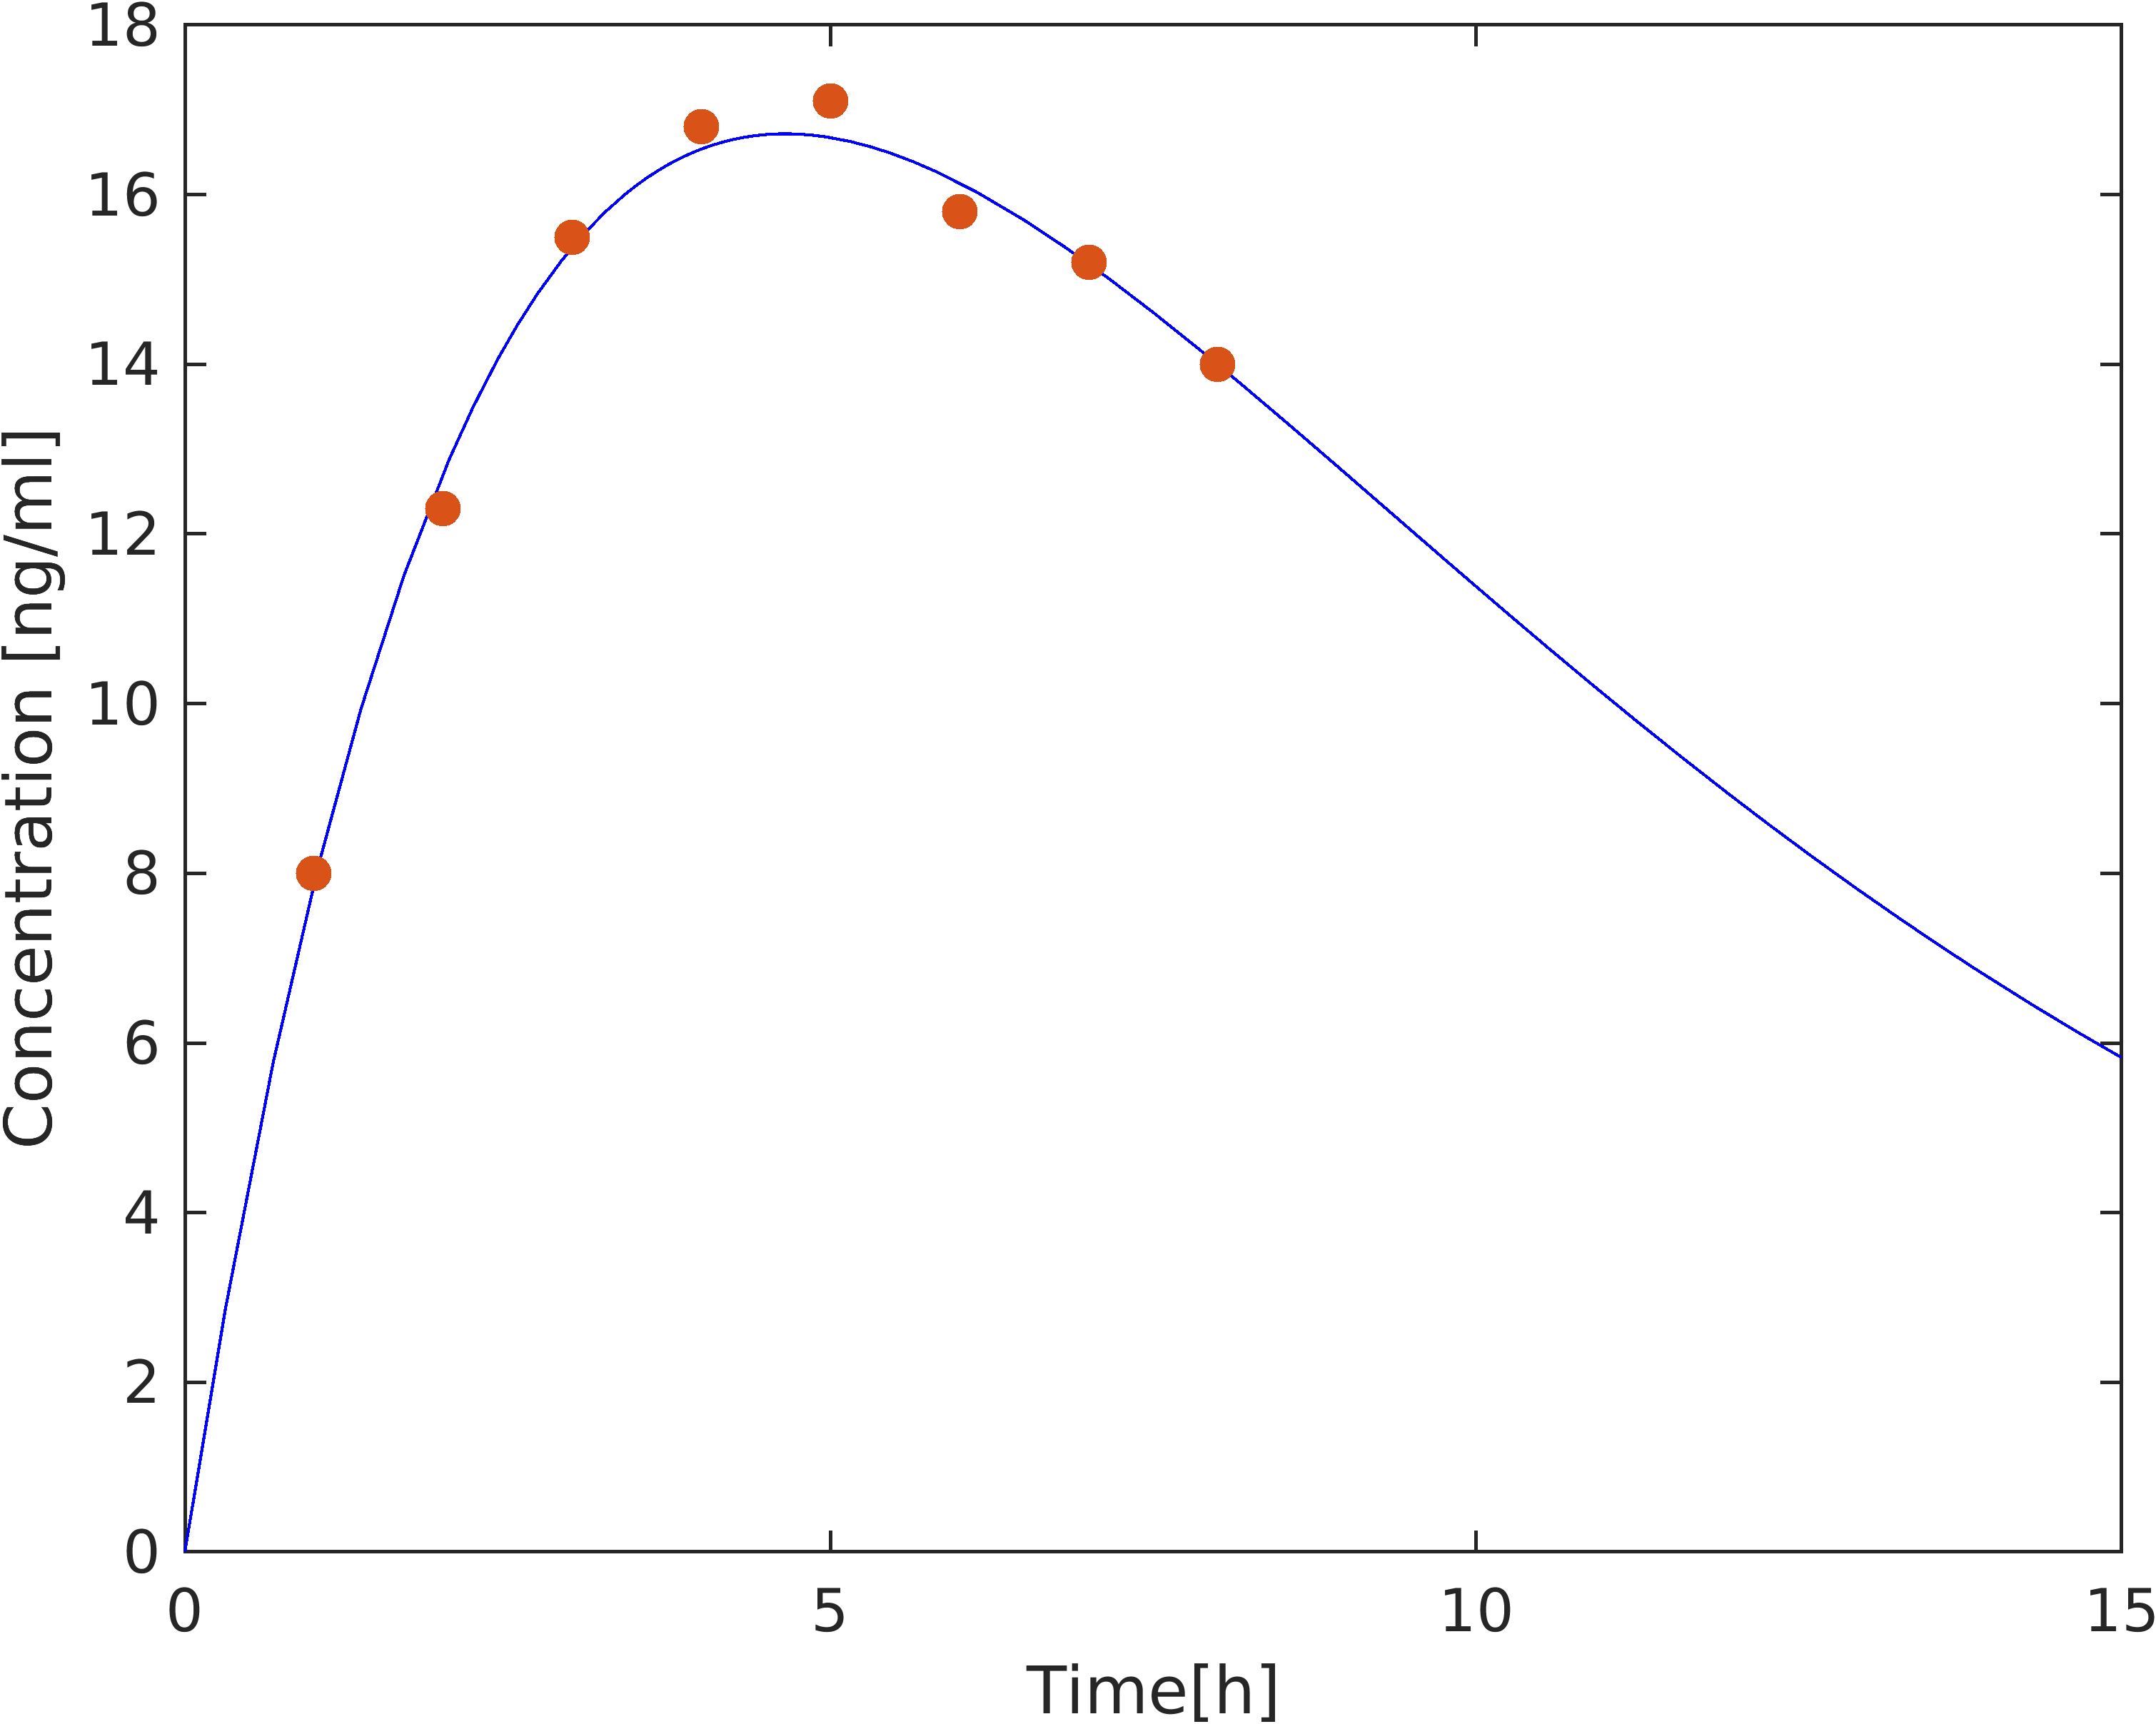
\includegraphics[width=0.8\textwidth]{img/Q2plot.png}
  \captionsetup{justification=centering}
  \caption{Data points and the fitted curve linearized regression}
\end{figure}

The curve equation $y = 9.77te^{-0.215t}$ demonstrates some limitations in accurately capturing the relationship between time and concentration in the given dataset. While it is evident that the curve tends to underestimate the concentration values across various time points close to the top point, it is important to note that the nature of curve fitting is often complex and dependent on multiple factors. Factors such as noise in the data, variability in measurements, and potential outliers can contribute to the observed deviations between the predicted and actual concentrations. Therefore, it is crucial to exercise caution when interpreting the fit of the curve and consider exploring alternative approaches or adjusting the curve equation to potentially achieve a better alignment with the underlying data patterns.



\subsubsection{Part B}

Given $\left(t_1, y_1\right),\left(t_2, y_2\right), \ldots \ldots .,\left(t_n, y_n\right)$, best fit $y=Ate^{Bt}$ to the data. The variables $A$ and $B$ are the constants of the exponential model. The residual at each data point $t_i$ is
\begin{equation}
E_i=y_i-At_ie^{Bt_i}
\end{equation}

The sum of the square of the residuals is
\begin{equation}
\begin{aligned}
S_r & =\sum_{i=1}^n E_i^2 \\
& =\sum_{i=1}^n\left(y_i-At_ie^{Bt_i}\right)^2
\end{aligned}
\end{equation}

To find the constants $A$ and $B$ of the exponential model, we find where $S_r$ is a local minimum or maximum by differentiating with respect to $A$ and $B$ and equating the resulting equations to zero.

\begin{subequations}
\begin{align}
\frac{\partial S_r}{\partial A}&=\sum_{i=1}^n 2\left(y_i-At_ie^{Bt_i}\right)\left(-t_ie^{Bt_i}\right)=0 \\
\frac{\partial S_r}{\partial B}&=\sum_{i=1}^n 2\left(y_i-At_ie^{Bt_i}\right)\left(-At_i^2e^{Bt_i}\right)=0
\end{align}
\end{subequations}

or
\begin{subequations}
\begin{align}
 -\sum_{i=1}^n \left(y_it_ie^{Bt_i}\right) + A\sum_{i=1}^n \left(t_i^2e^{2Bt_i}\right) &=0 \label{subeq1}\\
-\sum_{i=1}^n \left(y_iAt_i^2e^{Bt_i}\right) + \sum_{i=1}^n \left(A^2t_i^3e^{2Bt_i}\right) &=0  \label{subeq2}
\end{align}
\end{subequations}

Equations \ref{subeq1} and \ref{subeq2} are simultaneous nonlinear equations with constants $A$ and $B$. This is unlike linear regression where the equations to find the constants of the model are simultaneous but linear. In general, iterative methods (such as the Gauss-Newton iteration method, Method of Steepest Descent, Marquardt's Method, Direct search, etc) must be used to find values of $A$ and $B$.
However, in this case, from Equation \ref{subeq2}, $A$ can be written explicitly in terms of $B$ as
\begin{equation}
\label{aa}
A = \frac{\sum_{i=1}^n \left(y_it_ie^{Bt_i}\right)}{\sum_{i=1}^n \left(t_i^2e^{2Bt_i}\right)} \\    
\end{equation}

Rearrange the equation \ref{subeq2}:
\begin{equation}
    \label{fin}
    A\sum_{i=1}^n \left(t_i^3e^{2Bt_i}\right) = \sum_{i=1}^n \left(y_it_i^2e^{Bt_i}\right)\\
\end{equation}


Substituting Equation \ref{aa} in \ref{fin} gives

\begin{equation}
\label{son}
\frac{\sum_{i=1}^n \left(y_it_ie^{Bt_i}\right)}{\sum_{i=1}^n \left(t_i^2e^{2Bt_i}\right)} \sum_{i=1}^n \left(t_i^3e^{2Bt_i}\right) - \sum_{i=1}^n \left(y_it_i^2e^{Bt_i}\right) = 0\\    
\end{equation}

This equation is still a nonlinear equation in terms of $B$, and can be solved best by numerical methods such as the bisection method or the secant method.
We can now show that these values of $A$ and $B$, correspond to a local minimum, and since the above nonlinear equation has only one real solution, it corresponds to an absolute minimum. The solution of the equation \ref{son} by using an initial guess of zero and 'vpasolve' function of MATLAB is as follows:

\begin{equation}
    B = -0.215087
\end{equation}
Using this $B$ value and the equation \ref{aa} $A$ can be calculated as follows.
\begin{equation}
    A = 9.796928
\end{equation}
The function becomes:
\begin{equation}
    y = 9.796928te^{-0.215087t}
\end{equation}

To estimate the concentration at $t = 16$ hours, we substitute $t = 16$ into the model:

\begin{equation}
    y(16) = 5.01918
\end{equation}

\begin{figure}[H]
  \centering
  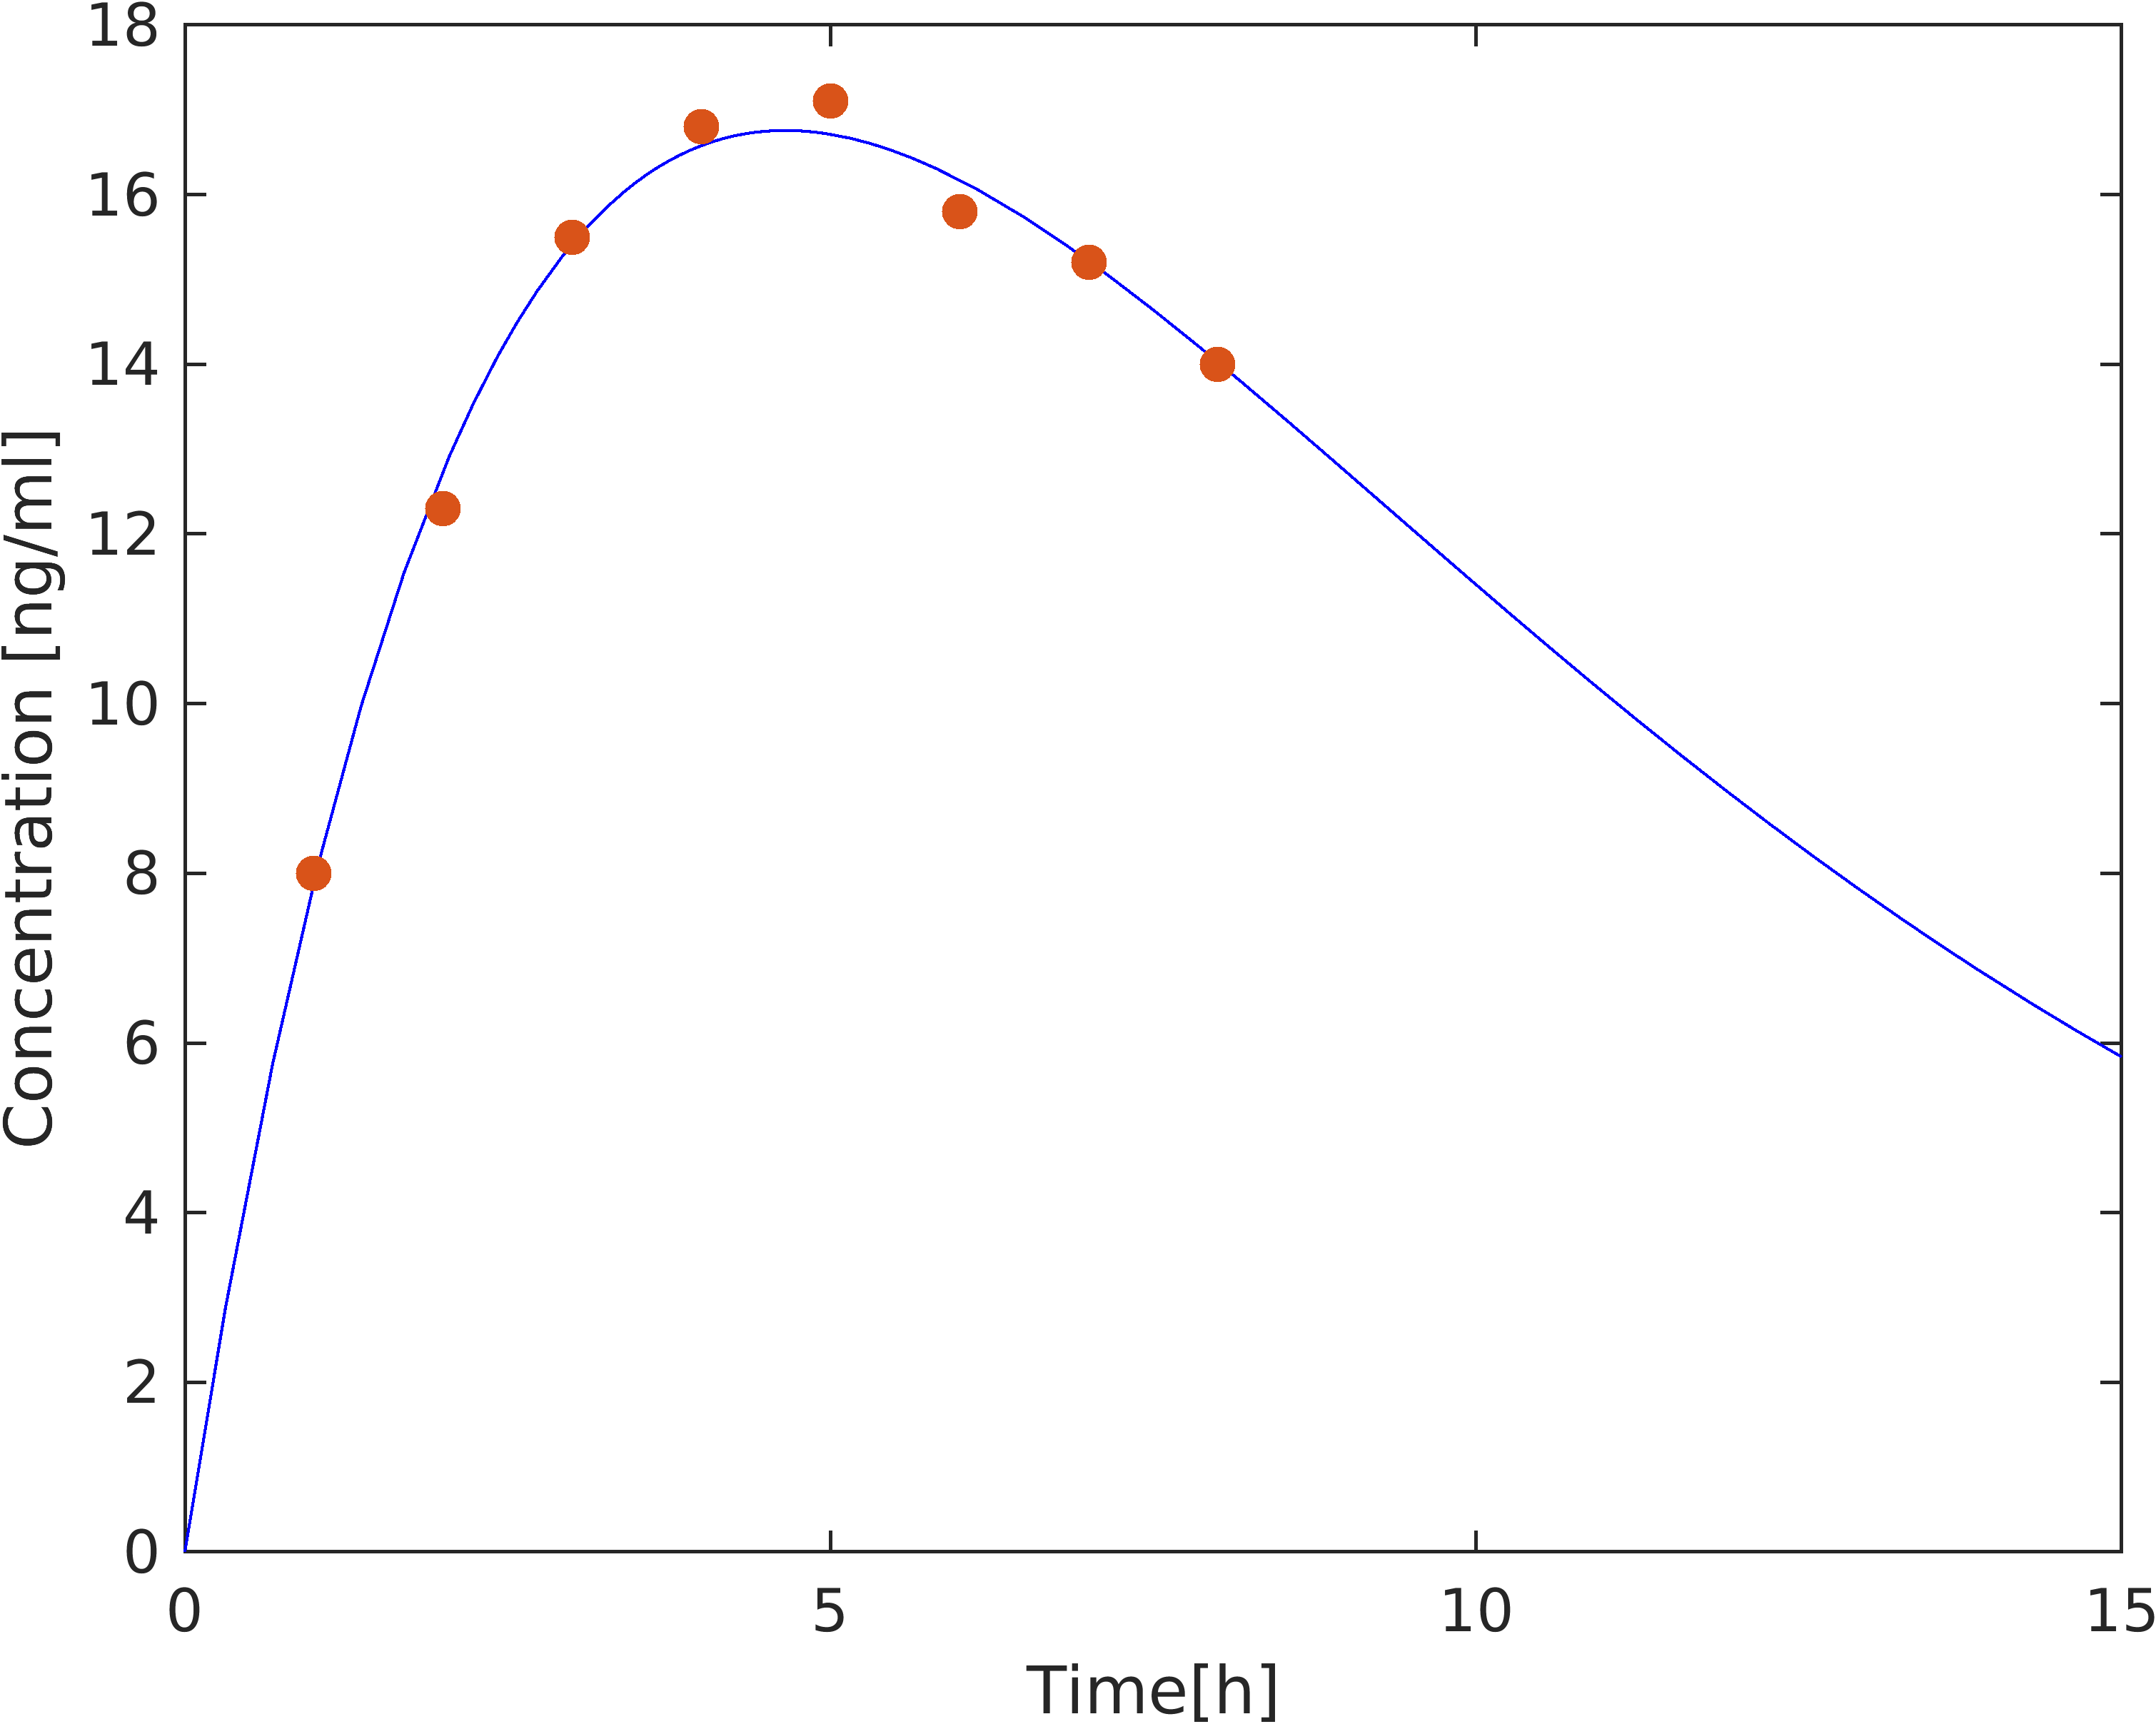
\includegraphics[width=0.8\textwidth]{img/Q2plot2.png}
  \captionsetup{justification=centering}
  \caption{Data points and the fitted curve non linear regression}
\end{figure}
The $r^2$ value:
$$ r^2 = 0.99111$$
As we can see from the plots and the functions the difference is not much. The linearizing method can be used to estimate the function. The quality of the fit for the linearized case and the non linear regression is similar. Depending on the desired accuracy both can be used. Both the $r^2$ values are close to each other and above 0.99 so we can say that the fit is quite good.

\subsubsection{Code}
\lstinputlisting[style=Matlab-editor, basicstyle=\mlttfamily\scriptsize]{Q2.m}


\newpage
\subsection{Question 6}
Generalized least square regression
\begin{equation} 
\begin{aligned}
& y=a_0 f_0+a_1 f_1+a_2 f_2+a_3 f_3 \cdots a_m f_m \\
& \eta=a_0 f_0+a_1 f_1+a_2 f_2
\end{aligned}
\end{equation}

Where:
\begin{equation} 
\begin{aligned}
& f_0=1 \\
& f_1=p \\
& f_2=h
\end{aligned}
\end{equation}

Construct the system
\begin{equation}
    Z^{\top} Z\{a\}=Z^{\top}\{\eta\}
    \label{system}
\end{equation}

Where:
\begin{equation}
Z=\left[\begin{array}{ccc}
f_0\left(p_1, h_1\right) & f_1\left(p_1, h_1\right) & f_2\left(p_1, h_1\right) \\
f_0\left(p_2, h_2\right) & f_1\left(p_2, h_2\right) & f_2\left(p_2, h_2\right) \\
\vdots & \vdots & \vdots \\
f_0\left(p_N, h_N\right) & f_1\left(p_N, h_N\right) & f_2\left(p_N, h_N\right)
\end{array}\right]_{N \times 3} \\
\end{equation}

\begin{equation}
    a=\left\{\begin{array}{l}
    a_0 \\
    a_1 \\
    a_2
\end{array}\right\}_{3 \times 1} \\
\end{equation}
\begin{equation}
    \eta=\left\{\begin{array}{l}
    \eta_0 \\
    \eta_1 \\
    \vdots \\
    \eta_N
\end{array}\right\}_{N \times 1}
\end{equation}


The $Z$ and $\eta$ are known.\\
\begin{equation}
   Z=\begin{bmatrix}
        1 & 16.4 & 80 \\ 
        1 & 22.4 & 80 \\ 
        1 & 29.8 & 80 \\ 
        1 & 23.9 & 110 \\ 
        1 & 32.1 & 110 \\ 
        1 & 41.0 & 110 \\ 
        1 & 38.8 & 145 \\ 
        1 & 46.2 & 145 \\ 
        1 & 59.7 & 145 \\ 
    \end{bmatrix} 
\end{equation}
\begin{equation}
\eta=\left\{\begin{array}{c}
75 \\
80 \\
85 \\
75 \\
80 \\
85 \\
75 \\
80 \\
85 \\
\end{array}\right\}
\end{equation}
The system \ref{system} can be solved as follows:
\begin{equation}
    \{a\}=(Z^{\top} Z)^{-1}Z^{\top}\{\eta\}
\end{equation}
The solution is as follows:
\begin{equation}
    a=\left\{\begin{array}{l}
    85.0731 \\
    0.5456 \\
    -0.2139
\end{array}\right\} \\
\end{equation}
The coefficient of determination $r^2$:

Calculate the total sum of squares (SST):
\begin{equation}
    \text{SST} = \sum (\eta_i - \bar{\eta})^2
\end{equation}
where $\eta_i$ is the observed efficiency, and $\bar{\eta}$ is the mean efficiency.

Calculate the sum of squares of residuals (SSR):
\begin{equation}
    \text{SSR} = \sum (\eta_i - \eta(P_i, h_i))^2
\end{equation}
where $ \eta (P_i, h_i)$ is the predicted efficiency obtained from the regression equation $\eta = a_0 + a_1P + a_2h$.

Calculate the coefficient of determination $r^2$:
\begin{equation}
r^2 = 1 - \frac{\text{SSR}}{\text{SST}}
\end{equation}

In this formulation, we can substitute the appropriate values and perform the calculations using the derived coefficient values from the least-squares fit to obtain the R-squared value.
The $r^2$ value:
$$ r^2 = 0.9348$$
Since the $r^2$ value is greater that 0.9 we can say that the quality of the fit is good. But depending on the required accuracy it can be bad or good. 

\newpage
\subsubsection{Code}
\lstinputlisting[style=Matlab-editor, basicstyle=\mlttfamily\scriptsize]{Q6.m}

\newpage

\subsection{Question 8}
\subsubsection{Part A}

a) To construct the finite divided difference table and determine the Newton's interpolating polynomial


\begin{table}[!ht]
    \centering
    \begin{tabular}{lccccccc}
    \hline
        $x$ & $f(x)$ & $f [ , ]$ & $f [ , ,]$ & $f [ , , ,]$ & $f [ , , , ,]$ & $f [ , , , , ,]$ & $f [ , , , , , ,]$ \\ \hline
        $x_0 = -1$ & -1 & A & G & L & P & T & V \\ 
        $x_1 = -0.96$ & -0.151 & B & H & M & R & U & \\ 
        $x_2 = -0.86$ & 0.894 & C & I & N & S & & \\ 
        $x_3 = -0.79$ & 0.986 & D & J & O & & & \\ 
        $x_4 = 0.22$ & 0.895 & E & K & & & & \\ 
        $x_5 = 0.5$ & 0.5 & F & & & & &  \\ 
        $x_6 = 0.93$ & -0.306 & & & & & & \\ \hline
    \end{tabular}
\end{table}

$f [ , ]$
\\
\begin{aligned}
& A=f\left[x_1, x_0\right]=\frac{f\left(x_1\right)-f\left(x_0\right)}{x_1-x_0}=21.2250\\
& B=f\left[x_2, x_1\right]=\frac{f\left(x_2\right)-f\left(x_1\right)}{x_2-x_1}=10.4500\\
& C=f\left[x_3, x_2\right]=\frac{f\left(x_3\right)-f\left(x_2\right)}{x_3-x_2}=1.3143\\
& D=f\left[x_4, x_3\right]=\frac{f\left(x_4\right)-f\left(x_3\right)}{x_4-x_3}=-0.09019\\
& E=f\left[x_5, x_4\right]=\frac{f\left(x_5\right)-f\left(x_4\right)}{x_5-x_4}=-1.4107\\
& F=f\left[x_6, x_5\right]=\frac{f\left(x_6\right)-f\left(x_5\right)}{x_6-x_5}=-1.8744\\
\end{aligned}
\\
\\
$f [ , ,]$\\
\\
\begin{aligned}
& G=f\left[x_2, x_1, x_0\right]=\frac{B-A}{x_2-x_0}= -76.9643\\
& H=f\left[x_3, x_2, x_1\right]=\frac{C-B}{x_3-x_1}= -53.7395\\
& I=f\left[x_4, x_3, x_2\right]=\frac{D-C}{x_4-x_2}= -1.3004\\
& J=f\left[x_5, x_4, x_3\right]=\frac{E-D}{x_5-x_3}= -1.0237\\
& K=f\left[x_6, x_5, x_4\right]=\frac{F-E}{x_6-x_4}= -0.6531\\
\end{aligned}
\\
\\
$f [ , , ,]$\\
\\
\begin{aligned}
& L=f\left[x_3, x_2, x_1, x_0\right]=\frac{H-G}{x_3-x_0}= 110.5942\\
& M=f\left[x_4, x_3, x_2, x_1\right]=\frac{I-H}{x_4-x_1}= 44.4399\\
& N=f\left[x_5, x_4, x_3, x_2\right]=\frac{J-I}{x_5-x_2}= 0.2034\\
& O=f\left[x_6, x_5, x_4, x_3\right]=\frac{K-J}{x_6-x_3}= 0.2155\\
\end{aligned}
\\
\\
$f [ , , , ,]$\\
\\
\begin{aligned}
& P=f\left[x_4, x_3, x_2, x_1, x_0\right]=\frac{M-L}{x_4-x_0}= -54.2248\\
& R=f\left[x_5 , x_4, x_3, x_2, x_1\right]=\frac{N-M}{x_5-x_1}= -30.2990\\
& S=f\left[x_6, x_5 , x_4, x_3, x_2\right]=\frac{O-N}{x_6-x_2}= 0.0067\\
\end{aligned}
\\
\\
$f [ , , , , ,]$\\
\\
\begin{aligned}
& T=f\left[x_5, x_4, x_3, x_2, x_1, x_0\right]=\frac{R-P}{x_5-x_0}= 15.9505\\
& U=f\left[x_6, x_5 , x_4, x_3, x_2, x_1\right]=\frac{S-R}{x_6-x_1}= 16.0348\\
\end{aligned}
\\
\\
$f [ , , , , , ,]$ \\
\begin{aligned}
& V=f\left[x_6, x_5, x_4, x_3, x_2, x_1, x_0\right]=\frac{U-T}{x_6-x_0}= 0.0436\\
\end{aligned}

\begin{equation}
\begin{split}
    f(x)= \\ 
    &\quad+0.0436 (x-0.5) (x-0.22) (x+0.79) (x+0.86) (x+0.96) (x+1) \\ &\quad+15.9505 (x-0.22) (x+0.79) (x+0.86) (x+0.96) (x+1) \\ 
    &\quad-54.2248 (x+0.79) (x+0.86) (x+0.96) (x+1) \\ 
    &\quad+110.594 (x+0.86) (x+0.96) (x+1) \\ 
    &\quad-76.9643 (x+0.96) (x+1)\\
    &\quad+21.225 (x+1) \\
    &\quad-1
\end{split}
\end{equation}

\begin{equation}
\begin{split}
    f(x)= \\ 
    &\quad+0.0436499 x^6\\ 
    &\quad+16.0767 x^5\\ 
    &\quad-0.0484021 x^4\\ 
    &\quad-20.1005 x^3\\ 
    &\quad+0.0168807 x^2\\ 
    &\quad+5.02946 x\\ 
    &\quad-0.00644606
\end{split}
\end{equation}

\begin{equation}
f(-0.2)= -0.856079
\end{equation}

\begin{figure}[H]
  \centering
  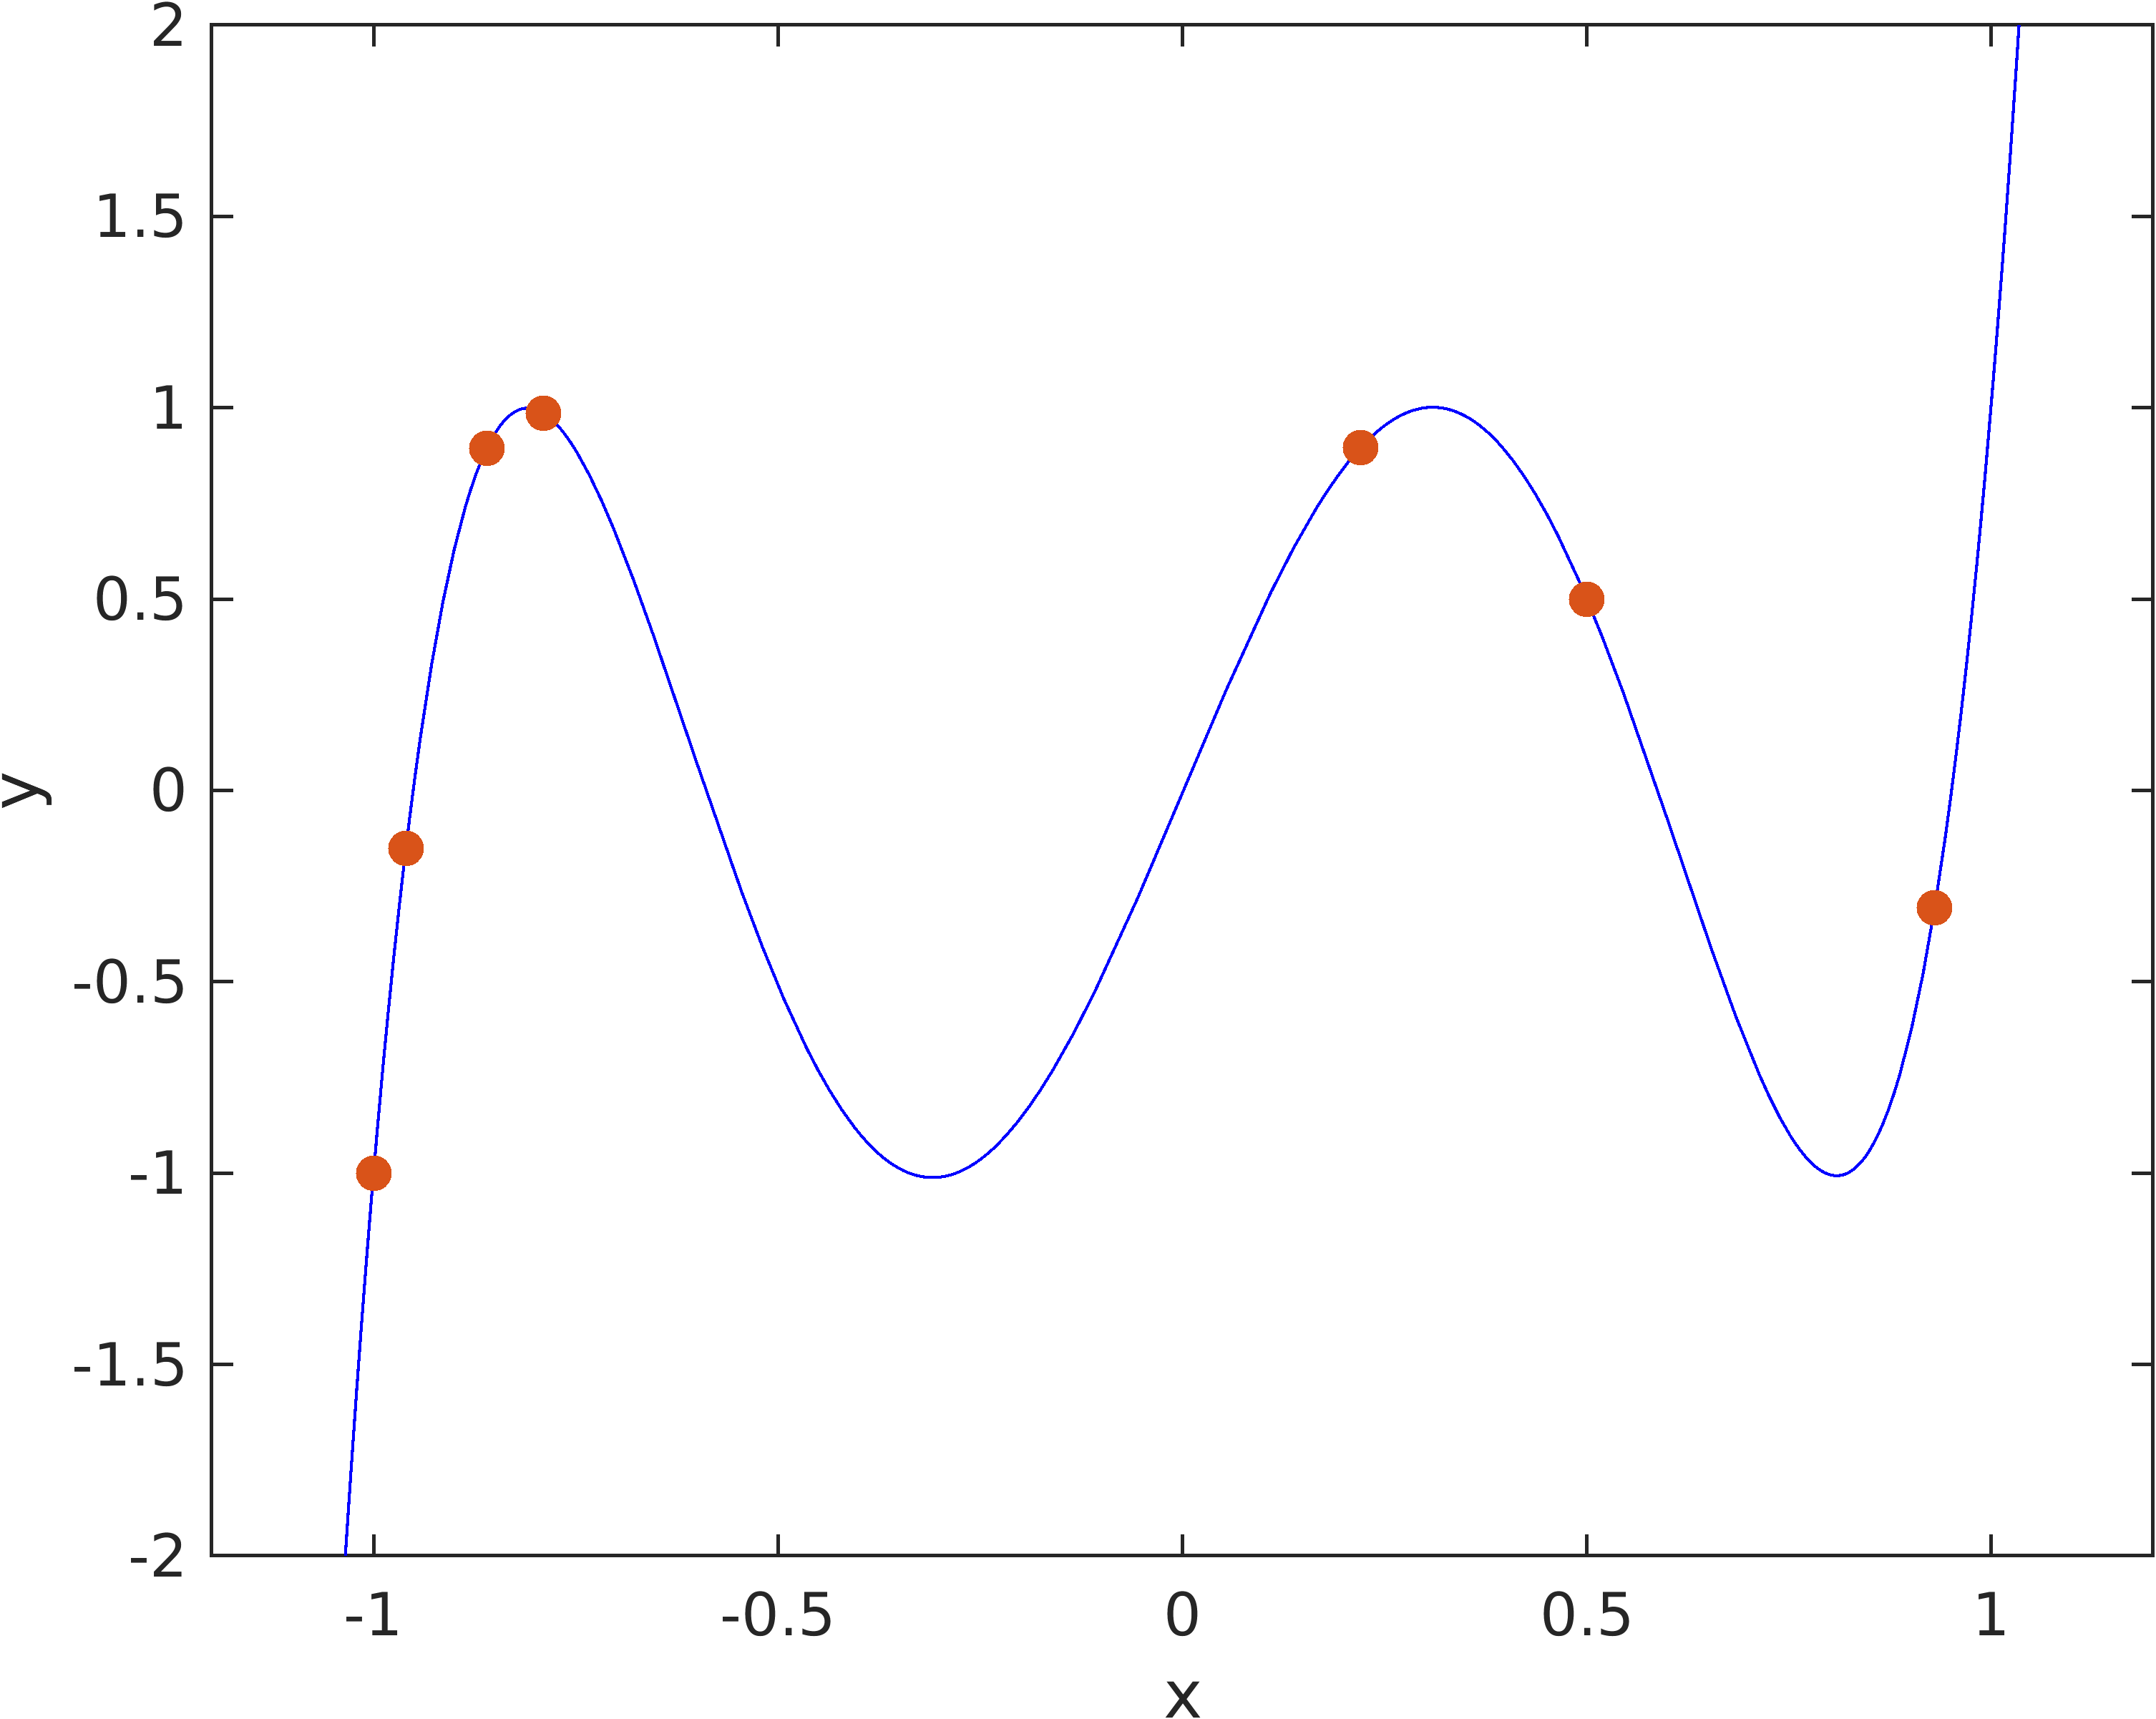
\includegraphics[width=0.8\textwidth]{img/Q8.png}
  \captionsetup{justification=centering}
  \caption{The polynomial fit for the the parts A and B}
\end{figure}

\subsubsection{Part B}
The Lagrangian interpolation is a method which makes it possible to find the equation of a polynomial function which passes through a series of n given points ${(x_0,y_0), (x_1,y_1), \dots, (x_n,y_n)}$

The Lagrange polynomial is calculated by the formula
\

\begin{equation}
    f(X) = \sum_{j=0}^n y_j \left(\prod_{i=0,i\neq j}^n \frac{X-x_i}{x_j-x_i} \right)
\end{equation}
For the given data points:

\begin{table}[!ht]
    \centering
    \begin{tabular}{cc}
    \hline
        $x_j$ & $y_j$ \\ \hline
        -1 & -1 \\ 
        -0.96 & -0.151 \\ 
        -0.86 & 0.894 \\ 
        -0.79 & 0.986 \\ 
        0.22 & 0.895 \\ 
        0.5 & 0.5 \\ 
        0.93 & -0.306 \\ \hline
    \end{tabular}
\end{table}
The sum is computed as follows

\[
\begin{aligned}
& \quad -1 \cdot \frac{{x - (-0.96)}}{{(-0.04)}} \cdot \frac{{x - (-0.86)}}{{(-0.14)}} \cdot \frac{{x - (-0.79)}}{{(-0.21)}} \cdot \frac{{x - 0.22}}{{(-1.22)}} \cdot \frac{{x - 0.5}}{{(-1.5)}} \cdot \frac{{x - 0.93}}{{(-1.93)}} \\
& \quad + (-0.151) \cdot \frac{{x - (-1)}}{{(0.04)}} \cdot \frac{{x - (-0.86)}}{{(-0.1)}} \cdot \frac{{x - (-0.79)}}{{(-0.17)}} \cdot \frac{{x - 0.22}}{{(-1.18)}} \cdot \frac{{x - 0.5}}{{(-1.46)}} \cdot \frac{{x - 0.93}}{{(-1.89)}} \\
& \quad + 0.894 \cdot \frac{{x - (-1)}}{{(0.14)}} \cdot \frac{{x - (-0.96)}}{{(0.1)}} \cdot \frac{{x - (-0.79)}}{{(-0.07)}} \cdot \frac{{x - 0.22}}{{(-1.08)}} \cdot \frac{{x - 0.5}}{{(-1.36)}} \cdot \frac{{x - 0.93}}{{(-1.79)}} \\
& \quad + 0.986 \cdot \frac{{x - (-1)}}{{(0.21)}} \cdot \frac{{x - (-0.96)}}{{(0.17)}} \cdot \frac{{x - (-0.86)}}{{(0.07)}} \cdot \frac{{x - 0.22}}{{(-1.01)}} \cdot \frac{{x - 0.5}}{{(-1.29)}} \cdot \frac{{x - 0.93}}{{(-1.72)}} \\
& \quad + 0.895 \cdot \frac{{x - (-1)}}{{(1.22)}} \cdot \frac{{x - (-0.96)}}{{(1.18)}} \cdot \frac{{x - (-0.86)}}{{(1.08)}} \cdot \frac{{x - (-0.79)}}{{(1.01)}} \cdot \frac{{x - 0.5}}{{(-0.28)}} \cdot \frac{{x - 0.93}}{{(-0.71)}} \\
& \quad + 0.5 \cdot \frac{{x - (-1)}}{{(1.5)}} \cdot \frac{{x - (-0.96)}}{{(1.46)}} \cdot \frac{{x - (-0.86)}}{{(1.36)}} \cdot \frac{{x - (-0.79)}}{{(1.29)}} \cdot \frac{{x - 0.22}}{{(0.28)}} \cdot \frac{{x - 0.93}}{{(-0.43)}} \\
& \quad + (-0.306) \cdot \frac{{x - (-1)}}{{(1.93)}} \cdot \frac{{x - (-0.96)}}{{(1.89)}} \cdot \frac{{x - (-0.86)}}{{(1.79)}} \cdot \frac{{x - (-0.79)}}{{(1.72)}} \cdot \frac{{x - 0.22}}{{(0.71)}} \cdot \frac{{x - 0.5}}{{(0.43)}}
\end{aligned}
\]

After simplification:

\begin{equation}
\begin{split}
    f(X) = 0.0436499 x^6+16.0767 x^5-0.0484021 x^4-20.1005 \\
    \quad x^3+0.0168807 x^2+5.02946 x-0.00644606
\end{split}
\end{equation}

\begin{equation}
f(-0.2)\to -0.856079
\end{equation}

\subsubsection{Part C}
Given a set of data points $(x_i, y_i)$ for $i = 0, 1, 2, \ldots, n$, where $x_0 < x_1 < x_2 < \ldots < x_n$, we want to construct a piecewise cubic polynomial function $S(x)$ that interpolates these points. The natural cubic spline interpolation ensures that the second derivative of $S(x)$ is zero at the endpoints, resulting in a smoother curve.

To construct the natural cubic spline, we divide the interval between each pair of consecutive points into subintervals and fit a cubic polynomial to each subinterval. Let $h_i = x_{i+1} - x_i$ be the width of the $i$th subinterval.

For each subinterval $[x_i, x_{i+1}]$, we define the cubic polynomial $S_i(x)$ as:

\[
S_i(x) = a_ix^3 + b_ix^2 + c_ix + d_i
\]

To determine the coefficients $a_i$, $b_i$, $c_i$, and $d_i$ for each subinterval, we solve the following system of equations:

\begin{align*}
S_i(x_i) &= y_i \\
S_i(x_{i+1}) &= y_{i+1} \\
S_i''(x_i) &= S_{i-1}''(x_i) \quad \text{(continuity of second derivative)} \\
S_i''(x_{i+1}) &= S_{i+1}''(x_{i+1}) \quad \text{(continuity of second derivative)}
\end{align*}

where $S_i''(x_i)$ and $S_i''(x_{i+1})$ are the second derivatives of $S_i(x)$ evaluated at $x_i$ and $x_{i+1}$, respectively. These equations can be solved by using techniques like the Gaussian elimination.

Once we determine the coefficients for each subinterval, we obtain the natural cubic spline function $S(x)$ by combining the individual cubic polynomials:

\[
S(x) = 
\begin{cases}
S_0(x), & \text{if } x_0 \leq x < x_1 \\
S_1(x), & \text{if } x_1 \leq x < x_2 \\
\ldots \\
S_{n-1}(x), & \text{if } x_{n-1} \leq x \leq x_n \\
\end{cases}
\]

The resulting natural cubic spline interpolation provides a smooth and continuous curve that passes through each data point.
For the given data points:

\begin{table}[!ht]
    \centering
    \begin{tabular}{cc}
    \hline
        $x_j$ & $y_j$ \\ \hline
        -1 & -1 \\ 
        -0.96 & -0.151 \\ 
        -0.86 & 0.894 \\ 
        -0.79 & 0.986 \\ 
        0.22 & 0.895 \\ 
        0.5 & 0.5 \\ 
        0.93 & -0.306 \\ \hline
    \end{tabular}
\end{table}


Let's solve the problem using the polynomial form \(S_i(x) = a_ix^3 + b_ix^2 + c_ix + d_i\) for each interval \([x_i, x_{i+1}]\).


Set up a system of equations for the coefficients \(a_i, b_i, c_i, d_i\) based on the given data.

For each interval, we have the following equations:

For the first interval \([-1, -0.96]\):
\[S_1(x) = a_1x^3 + b_1x^2 + c_1x + d_1\]
\[S_1(-1) = -a_1 + b_1 - c_1 + d_1 = -1\]
\[S_1(-0.96) = -a_1(0.96)^3 + b_1(0.96)^2 - c_1(0.96) + d_1 = -0.151\]

For the second interval \([-0.96, -0.86]\):
\[S_2(x) = a_2x^3 + b_2x^2 + c_2x + d_2\]
\[S_2(-0.96) = -a_2(0.96)^3 + b_2(0.96)^2 - c_2(0.96) + d_2 = -0.151\]
\[S_2(-0.86) = -a_2(0.86)^3 + b_2(0.86)^2 - c_2(0.86) + d_2 = 0.894\]

For the third interval \([-0.86, -0.79]\):
\[S_3(x) = a_3x^3 + b_3x^2 + c_3x + d_3\]
\[S_3(-0.86) = -a_3(0.86)^3 + b_3(0.86)^2 - c_3(0.86) + d_3 = 0.894\]
\[S_3(-0.79) = -a_3(0.79)^3 + b_3(0.79)^2 - c_3(0.79) + d_3 = 0.986\]

For the fourth interval \([-0.79, 0.22]\):
\[S_4(x) = a_4x^3 + b_4x^2 + c_4x + d_4\]
\[S_4(-0.79) = -a_4(0.79)^3 + b_4(0.79)^2 - c_4(0.79) + d_4 = 0.986\]
\[S_4(0.22) = a_4(0.22)^3 + b_4(0.22)^2 + c_4(0.22) + d_4 = 0.895\]

For the fifth interval \([0.22, 0.5]\):
\[S_5(x) = a_5x^3 + b_5x^2 + c_5x + d_5\]
\[S_5(0.22) = a_5(0.22)^3 + b_5(0.22)^2 + c_5(0.22) + d_5 = 0.895\]
\[S_5(0.5) = a_5(0.5)^3 + b_5(0.5)^2 + c_5(0.5) + d_5 = 0.5\]

For the sixth interval \([0.5, 0.93]\):
\[S_6(x) = a_6x^3 + b_6x^2 + c_6x + d_6\]
\[S_6(0.5) = a_6(0.5)^3 + b_6(0.5)^2 + c_6(0.5) + d_6 = 0.5\]
\[S_6(0.93) = a_6(0.93)^3 + b_6(0.93)^2 + c_6(0.93) + d_6 = -0.306\]

To find the first and second derivatives of the cubic splines, we can differentiate the polynomial form \(S_i(x) = a_ix^3 + b_ix^2 + c_ix + d_i\) with respect to \(x\).

Let's consider each interval \([x_i, x_{i+1}]\) and calculate the derivatives.

For the first interval \([-1, -0.96]\), the polynomial form is \(S_1(x) = a_1x^3 + b_1x^2 + c_1x + d_1\). Differentiating \(S_1(x)\) once gives us:

\[S_1'(x) = 3a_1x^2 + 2b_1x + c_1\]

Differentiating \(S_1(x)\) twice gives us the second derivative:

\[S_1''(x) = 6a_1x + 2b_1\]

For the second interval \([-0.96, -0.86]\), the polynomial form is \(S_2(x) = a_2x^3 + b_2x^2 + c_2x + d_2\). Differentiating \(S_2(x)\) once gives us:

\[S_2'(x) = 3a_2x^2 + 2b_2x + c_2\]

Differentiating \(S_2(x)\) twice gives us the second derivative:

\[S_2''(x) = 6a_2x + 2b_2\]

Similarly, we can differentiate the polynomials for the remaining intervals to find their corresponding first and second derivatives.

For the third interval \([-0.86, -0.79]\):
\[S_3'(x) = 3a_3x^2 + 2b_3x + c_3\]
\[S_3''(x) = 6a_3x + 2b_3\]

For the fourth interval \([-0.79, 0.22]\):
\[S_4'(x) = 3a_4x^2 + 2b_4x + c_4\]
\[S_4''(x) = 6a_4x + 2b_4\]

For the fifth interval \([0.22, 0.5]\):
\[S_5'(x) = 3a_5x^2 + 2b_5x + c_5\]
\[S_5''(x) = 6a_5x + 2b_5\]

For the sixth interval \([0.5, 0.93]\):
\[S_6'(x) = 3a_6x^2 + 2b_6x + c_6\]
\[S_6''(x) = 6a_6x + 2b_6\]

Let's equate the first and second derivatives of the cubic splines at the midpoint of each interval.

For the first interval \([-1, -0.96]\), the midpoint is \(-0.98\). We equate the first and second derivatives at this point:

\[S_1'(-0.98) = S_2'(-0.98)\]
\[3a_1(-0.98)^2 + 2b_1(-0.98) + c_1 = 3a_2(-0.98)^2 + 2b_2(-0.98) + c_2\]

For the second interval \([-0.96, -0.86]\), the midpoint is \(-0.91\). We equate the first and second derivatives at this point:

\[S_2'(-0.91) = S_3'(-0.91)\]
\[3a_2(-0.91)^2 + 2b_2(-0.91) + c_2 = 3a_3(-0.91)^2 + 2b_3(-0.91) + c_3\]

For the third interval \([-0.86, -0.79]\), the midpoint is \(-0.825\). We equate the first and second derivatives at this point:

\[S_3'(-0.825) = S_4'(-0.825)\]
\[3a_3(-0.825)^2 + 2b_3(-0.825) + c_3 = 3a_4(-0.825)^2 + 2b_4(-0.825) + c_4\]

For the fourth interval \([-0.79, 0.22]\), the midpoint is \(0.215\). We equate the first and second derivatives at this point:

\[S_4'(0.215) = S_5'(0.215)\]
\[3a_4(0.215)^2 + 2b_4(0.215) + c_4 = 3a_5(0.215)^2 + 2b_5(0.215) + c_5\]

For the fifth interval \([0.22, 0.5]\), the midpoint is \(0.36\). We equate the first and second derivatives at this point:

\[S_5'(0.36) = S_6'(0.36)\]
\[3a_5(0.36)^2 + 2b_5(0.36) + c_5 = 3a_6(0.36)^2 + 2b_6(0.36) + c_6\]

By equating the first and second derivatives at the midpoints, we ensure smoothness and continuity between adjacent intervals of the cubic splines.

From these equations we can construct a $4n$ by $4n$ system. By solving the system of equations, we can obtain the values of the coefficients. Once we have the coefficients, we can interpolate for \(y(-0.2)\) by finding the corresponding spline interval and substituting the value of \(x\) into the corresponding spline equation.

Please note that solving the system of equations requires numerical methods, such as matrix inversion or Gaussian elimination. The detailed calculations would involve substantial numerical computations, which are better suited for programming or computational tools.
\\
\\
By solving the system we can obtain the coefficients and the result is as follows:
\\

f(x) = \begin{cases}-8.0655 \cdot 10^{2}\cdot x^3 -2.4196 \cdot 10^{3}\cdot x^2 -2.3971 \cdot 10^{3}\cdot x -7.8503 \cdot 10^{2}, & \text{if } x \in [-1,-0.96], \\1.4845 \cdot 10^{2}\cdot x^3 + 3.3075 \cdot 10^{2}\cdot x^2 + 2.4325 \cdot 10^{2}\cdot x + 5.9888 \cdot 10^{1}, & \text{if } x \in (-0.96,-0.86], \\2.5131 \cdot 10^{2}\cdot x^3 + 5.9612 \cdot 10^{2}\cdot x^2 + 4.7147 \cdot 10^{2}\cdot x + 1.2531 \cdot 10^{2}, & \text{if } x \in (-0.86,-0.79], \\-7.2399 \cdot 10^{-1}\cdot x^3 -1.1922\cdot x^2 -4.0859 \cdot 10^{-1}\cdot x + 1.0503, & \text{if } x \in (-0.79,0.22], \\1.2139\cdot x^3 -2.4712\cdot x^2 -1.2721 \cdot 10^{-1}\cdot x + 1.0297, & \text{if } x \in (0.22,0.5], \\5.0415 \cdot 10^{-1}\cdot x^3 -1.4066\cdot x^2 -6.5951 \cdot 10^{-1}\cdot x + 1.1184, & \text{if } x \in (0.5,0.93].\end{cases}
\\
The solution is as follows
$$f(-0.2)=1.0901$$
\\
\\

\begin{figure}[H]
\begin{center}
    \begin{tikzpicture}
    
    		\pgfplotsset{
    			scale only axis,
    		}
    
    		\begin{axis}[
    			xlabel=$x$,
    			ylabel=$y$,
    			samples=100,
    			]\addplot [only marks] table {
    -1 -1
    -0.96 -0.151
    -0.86 0.894
    -0.79 0.986
    0.22 0.895
    0.5 0.5
    0.93 -0.306
    };
    
    			
    			\addplot[][domain=-1:-0.96]{+-806.5453890500314*x^3+-2419.6361671500945*x^2+-2397.1206945276144*x^1+-785.0299164275514*x^0};
    			\addplot[][domain=-0.96:-0.86]{+148.44899135604777*x^3+330.7476484194138*x^2+243.24776841911353*x^1+59.887991715401505*x^0};
    			\addplot[][domain=-0.86:-0.79]{+251.30673577722385*x^3+596.1206290260482*x^2+471.46853174081906*x^1+125.31127720095708*x^0};
    			\addplot[][domain=-0.79:0.22]{+-0.7239880125753181*x^3+-1.192186355775935*x^2+-0.40859241082196185*x^1+1.0503011743582888*x^0};
    			\addplot[][domain=0.22:0.5]{+1.2138819568393402*x^3+-2.4711805355896095*x^2+-0.12721369126295348*x^1+1.0296667349239617*x^0};
    			\addplot[][domain=0.5:0.93]{+0.504153178550852*x^3+-1.406587368156877*x^2+-0.6595102749793197*x^1+1.1183828322100227*x^0};		\end{axis}
    
    	\end{tikzpicture}
\end{center}
  \captionsetup{justification=centering}
  \caption{The spline fit}
\end{figure}

\subsubsection{Part D}
To achieve similar outcomes as in the previous sections, two common interpolation methods, namely Newton's interpolating polynomial and Lagrange interpolating polynomial, were utilized. These methods provide a unified polynomial representation that accurately captures the entire dataset. While the mathematical techniques employed differ, both approaches ensure the interpolation of all the given data points.

In contrast, part c introduced a slight deviation from the previous methods. Instead of relying on polynomial interpolation, natural cubic splines were employed to interpolate the dataset. This technique involves breaking down the data into smaller intervals and employing piecewise cubic polynomials to estimate the values within each interval. Consequently, the interpolation for $y(-0.2)$ may exhibit slight variations compared to the interpolations obtained in parts a and b.

Despite these slight variations, all three methods aim to approximate the underlying relationship among the provided data points. The choice between Newton's interpolating polynomial, Lagrange interpolating polynomial, and natural cubic splines hinges on specific considerations, including desired smoothness, continuity, and the ability to handle diverse data characteristics.

Also note that since the curves are same for the part A and part B there is only a single figure for both of them.

\subsubsection{Code}
\lstinputlisting[style=Matlab-editor, basicstyle=\mlttfamily\scriptsize]{Q8.m}

\section{Question 13}
To perform bi-quadratic interpolation first we select 3 sets of points and perform quadratic interpolation among the set. After that perform another quadratic interpolation among the new points. 
The sets are:
\begin{center}
Set 1: $(x_2, y_2)$, $(x_4, y_2)$, $(x_6, y_2)$\\
Set 2: $(x_2, y_4)$, $(x_4, y_4)$, $(x_6, y_4)$\\
Set 3: $(x_2, y_6)$, $(x_4, y_6)$, $(x_6, y_6)$\\    
\end{center}

\begin{comment}
    For the set 1:\\
    f_1(x)= \\ \begin{array}{c} 0.705 (x-4) (x-2)-5.495 (x-2)+64.49 \\ = \\ 
    0.705 x^2-9.725 x+81.12 \end{array}
    For the set 2:\\
    f_2(x)= \\ \begin{array}{c} 0.88375 (x-4) (x-2)-5.235 (x-2)+48.9 \\ = \\ 0.88375 x^2-10.5375 x+66.44 \end{array}
    For the set 3:\\
    f_3(x)= \\ \begin{array}{c} 0.63375 (x-4) (x-2)-4.195 (x-2)+38.78 \\ = \\ 0.63375 x^2-7.9975 x+52.24 \end{array}
    
    Now compute the functions for $x = 3$ and $x = 4.3$
    
    f_1(3) & = & 58.29
    f_2(3) & = & 42.7813
    f_3(3) & = & 33.9513
    
    2, 58.29
    4, 42.7813
    6, 33.9513
    
    
    f(x)= \\ \begin{array}{c} 0.834837 (x-4) (x-2)-7.75435 (x-2)+58.29 \\ = \\ 0.834837 x^2-12.7634 x+80.4774 \end{array}
    
    f(3.2) & = & 48.1833
    
    f_1(4.3) & = & 52.338
    f_2(4.3) & = & 37.4693
    f_3(4.3) & = & 29.5688
    
    f(x)= \\ \begin{array}{c} 0.871025 (x-4) (x-2)-7.43435 (x-2)+52.338 \\ = \\ 0.871025 x^2-12.6605 x+74.1749 \end{array}
    
    f(2.7) & = & 46.3413
    
    52.338
    37.4693
    29.5688
\end{comment}

The calculations for the quadratic interpolations are as follows:

For Set 1: 
$$(x_2, t_{22}), (x_4, t_{42}), (x_6, t_{62})$$

To find $f_1(x)$ we have the points 
$$(2, 64.49), (4, 64.49), (6, 64.49)$$

Using the quadratic interpolation formula:
\begin{equation}
    f_1(x) = t_{22} \cdot \frac{(x-x_4)(x-x_6)}{(x_2-x_4)(x_2-x_6)} + t_{42} \cdot \frac{(x-x_2)(x-x_6)}{(x_4-x_2)(x_4-x_6)} + t_{62} \cdot \frac{(x-x_2)(x-x_4)}{(x_6-x_2)(x_6-x_4)}
\end{equation}

Plugging in the given values, we get:
\begin{equation}
    f_1(x) = 64.49 \cdot \frac{(x-4)(x-6)}{(2-4)(2-6)} + 64.49 \cdot \frac{(x-2)(x-6)}{(4-2)(4-6)} + 64.49 \cdot \frac{(x-2)(x-4)}{(6-2)(6-4)}
\end{equation}

Simplifying the expression:
\begin{equation}
    f_1(x) = 0.705 (x-4)(x-6) - 5.495(x-2) + 64.49
\end{equation}

Expanding and simplifying further:
\begin{equation}
    f_1(x) = 0.705x^2 - 9.725x + 81.12
\end{equation}

For Set 2: 
$$(x_2, t_{24}), (x_4, t_{44}), (x_6, t_{64})$$

To find $f_2(x)$:
We have the points 
$$(2, 48.9), (4, 48.9), (6, 48.9)$$

Using the quadratic interpolation formula:
\begin{equation}
    f_2(x) = y_2 \cdot \frac{(x-x_4)(x-x_6)}{(x_2-x_4)(x_2-x_6)} + y_4 \cdot \frac{(x-x_2)(x-x_6)}{(x_4-x_2)(x_4-x_6)} + y_6 \cdot \frac{(x-x_2)(x-x_4)}{(x_6-x_2)(x_6-x_4)}
\end{equation}

Plugging in the given values, we get:
\begin{equation}
    f_2(x) = 48.9 \cdot \frac{(x-4)(x-6)}{(2-4)(2-6)} + 48.9 \cdot \frac{(x-2)(x-6)}{(4-2)(4-6)} + 48.9 \cdot \frac{(x-2)(x-4)}{(6-2)(6-4)}
\end{equation}


Simplifying the expression:
\begin{equation}
    f_2(x) = 0.88375 (x-4)(x-6) - 5.235(x-2) + 48.9
\end{equation}

Expanding and simplifying further:
\begin{equation}
    f_2(x) = 0.88375x^2 - 10.5375x + 66.44
\end{equation}

For Set 3:
$$(x_2, t_{26}), (x_4, t_{46}), (x_6, t_{66})$$

To find $f_3(x)$:
We have the points 
$$(2, 38.78), (4, 38.78), (6, 38.78)$$$

Using the quadratic interpolation formula:
\begin{equation}
    f_3(x) = y_2 \cdot \frac{(x-x_4)(x-x_6)}{(x_2-x_4)(x_2-x_6)} + y_4 \cdot \frac{(x-x_2)(x-x_6)}{(x_4-x_2)(x_4-x_6)} + y_6 \cdot \frac{(x-x_2)(x-x_4)}{(x_6-x_2)(x_6-x_4)}
\end{equation}

Plugging in the given values, we get:
\begin{equation}
    f_3(x) = 38.78 \cdot \frac{(x-4)(x-6)}{(2-4)(2-6)} + 38.78 \cdot \frac{(x-2)(x-6)}{(4-2)(4-6)} + 38.78 \cdot \frac{(x-2)(x-4)}{(6-2)(6-4)}
\end{equation}


Simplifying the expression:
\begin{equation}
    f_3(x) = 0.63375 (x-4)(x-6) - 4.195(x-2) + 38.78
\end{equation}


Expanding and simplifying further:
\begin{equation}
    f_3(x) = 0.63375x^2 - 7.9975x + 52.24
\end{equation}


Now, let's compute the values of these functions for $x = 3$ and $x = 4.3$:

For $x = 3$:
\begin{subequations}
\begin{align}
f_1(3) &= 0.705(3)^2 - 9.725(3) + 81.12 = 58.29 \\
f_2(3) &= 0.88375(3)^2 - 10.5375(3) + 66.44 = 42.7813 \\
f_3(3) &= 0.63375(3)^2 - 7.9975(3) + 52.24 = 33.9513
\end{align}
\end{subequations}

For $x = 4.3$:
\begin{subequations}
\begin{align}
f_1(4.3) &= 0.705(4.3)^2 - 9.725(4.3) + 81.12 = 52.338 \\
f_2(4.3) &= 0.88375(4.3)^2 - 10.5375(4.3) + 66.44 = 37.4693 \\
f_3(4.3) &= 0.63375(4.3)^2 - 7.9975(4.3) + 52.24 = 29.5688
\end{align}
\end{subequations}

To find $g_1(x)$:
We have the points 
$$(58.29, 2), (42.7813, 4), (33.9513, 6)$$$

Using these points, we can construct the quadratic interpolation function using the formula:
\begin{equation}
    g_1(x) = y_1 \cdot \frac{(x - x_2)(x - x_3)}{(x_1 - x_2)(x_1 - x_3)} + y_2 \cdot \frac{(x - x_1)(x - x_3)}{(x_2 - x_1)(x_2 - x_3)} + y_3 \cdot \frac{(x - x_1)(x - x_2)}{(x_3 - x_1)(x_3 - x_2)}
\end{equation}


Plugging in the given values, we have:
\begin{equation}
    g_1(x) = 58.29 \cdot \frac{(x - 4)(x - 6)}{(2 - 4)(2 - 6)} + 42.7813 \cdot \frac{(x - 2)(x - 6)}{(4 - 2)(4 - 6)} + 33.9513 \cdot \frac{(x - 2)(x - 4)}{(6 - 2)(6 - 4)}
\end{equation}


Simplifying further:
\begin{equation}
    g_1(x) = 0.834837 (x - 4)(x - 6) - 7.75435 (x - 2) + 58.29
\end{equation}

Therefore, the quadratic interpolation function for the given points is:
\begin{equation}
    g_1(x) = 0.834837 x^2-12.7634 x+80.4774
\end{equation}


To find $g_2(x)$ we have points  $$(52.338, 2), (37.4693,  4), and (29.5688, 6)$$ 

Using these points, we can construct the quadratic interpolation function using the formula:
\begin{equation}
    g_2(x) = y_1 \cdot \frac{(x - x_2)(x - x_3)}{(x_1 - x_2)(x_1 - x_3)} + y_2 \cdot \frac{(x - x_1)(x - x_3)}{(x_2 - x_1)(x_2 - x_3)} + y_3 \cdot \frac{(x - x_1)(x - x_2)}{(x_3 - x_1)(x_3 - x_2)}
\end{equation}


Plugging in the given values, we have:
\begin{equation}
    g_2(x) = 52.338 \cdot \frac{(x - 4)(x - 6)}{(2 - 4)(2 - 6)} + 37.4693 \cdot \frac{(x - 2)(x - 6)}{(4 - 2)(4 - 6)} + 29.5688 \cdot \frac{(x - 2)(x - 4)}{(6 - 2)(6 - 4)}
\end{equation}


Simplifying further:
\begin{equation}
    g_2(x) = 0.63375 (x-4) (x-2)-4.195 (x-2)+38.78
\end{equation}


Therefore, the quadratic interpolation function for the given points is:
\begin{equation}
    g_2(x) = 0.871025 -12.6605x^2 x+74.1749
\end{equation}


At final we have temperatures for the desired points.

$$ T(3, 3.2) = 48.1833$$
$$ T(4.3, 2.7) = 46.3413$$

\newpage
\section{Discussion}
Throughout the homework assignment, I gained valuable insights and skills in regression and interpolation techniques. Question two provided a comprehensive understanding of linearizing curves, performing both linear and non-linear regression analyses, and assessing the quality of fit using the r^2 value. This knowledge expanded my ability to model and analyze relationships between variables.

In question six, I delved into generalized regression, which broadened my repertoire beyond traditional regression methods. This allowed me to explore a wider range of mathematical models, enhancing my analytical capabilities and enabling me to handle more complex datasets.

Question eight proved to be an enlightening exercise as I compared Newton and Lagrange interpolation methods. Through this comparison, I learned that although their goal is the same—to fit a polynomial—they employ distinct approaches. Additionally, I discovered the advantages of cubic splines, which offer smoother and more visually appealing curve representations compared to conventional interpolation techniques. This understanding of cubic splines provides me with a valuable tool for handling data that requires a continuous and aesthetically pleasing curve.

Lastly, in question thirteen, I acquired the ability to perform bi-quadratic interpolation. This technique enabled me to estimate values between known data points using a two-dimensional polynomial function. The knowledge gained here is particularly valuable when dealing with limited or irregularly distributed data points.

These experiences have significantly deepened my understanding of regression and interpolation techniques, equipping me with a versatile skill set for analyzing and interpreting data. I am now better prepared to apply these mathematical tools in real-world scenarios across a variety of disciplines, enhancing my problem-solving abilities and enabling me to make informed decisions based on the strengths and limitations of different approaches.

\section{Conclusion}

In conclusion, the homework assignment discussed in this paragraph offers students an enriching opportunity to explore and master a diverse range of regression and interpolation techniques. By delving into linear and non-linear regression, generalized regression, polynomial fitting using Newton and Lagrange methods, natural cubic spline interpolation, and bi-quadratic interpolation, students gain practical experience and a deeper understanding of these essential mathematical tools. These exercises not only enhance their analytical capabilities but also equip them with the skills to handle and interpret real-world data. By engaging with these tasks, students develop the confidence and proficiency needed to apply regression and interpolation techniques in various fields. Overall, this assignment serves as a stepping stone for students to further their mathematical knowledge and cultivate valuable problem-solving skills.


\end{document}
